\documentclass{standalone}
\usepackage{mintikz}

\tikzset{every picture/.style={thick}}

\begin{document}
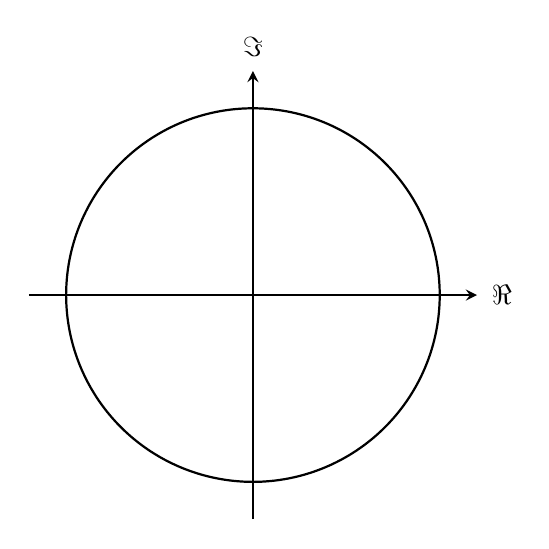
\begin{tikzpicture}[]
	\begin{axis}[
			axis lines=center,
			axis equal image,
			xtick=\empty, ytick=\empty,
			enlargelimits=true,
			xlabel=$\Re$, ylabel=$\Im$,
			every axis x label/.style={
					at={(ticklabel* cs:1.01)},
					anchor=west,
				},
			every axis y label/.style={
					at={(ticklabel* cs:1.01)},
					anchor=south,
				},
			clip=false,
		]
		\coordinate (O) at (0,0);
		\coordinate (X) at (1,0);
		\coordinate (Y) at (0,1);
		\coordinate (F) at ({cos(deg(pi/12))},{sin(deg(pi/12))});
		\coordinate (T) at ({cos(deg(pi/6))},{sin(deg(pi/6))});

		% \draw[dashed] (T) -- (T|-X) coordinate(TX);

		\addplot[data cs=polar,
			domain=0:360,
			samples=360,
			smooth,
			% flch={pos=0.1}
		]
		(x,{cos(x)^2+sin(x)^2});
		% \draw[-Stealth]
		% (0,0) -- (T)
		% node[midway, above] {$A$}
		% ;
		% Draw angles
		% \pic[angle radius=1cm, angle eccentricity=1.5,
		% 	draw, ->, "$\phi(t)$"]
		% {angle=X--O--T};
		% \pic[angle radius=2.5cm, angle eccentricity=1.1,
		% 	limegreen,
		% 	draw, ->, "$\f_0$"]
		% {angle=X--O--F};
		% \pic[angle radius=2.5cm, angle eccentricity=1.1,
		% 	cornflowerblue,
		% 	draw, ->, "$\wt$"]
		% {angle=F--O--T};
		% Grandeurs
		% \node[below=0.15cm, inner sep=0] (Oo) at (O) {};
		% \node[below=0.15cm, inner sep=0] (TXo) at (TX) {};
		% \draw[<->, firebrick] (Oo) --
		% node[below, midway, sloped]{$s(t)$}
		% (TXo);
	\end{axis}
\end{tikzpicture}
\end{document}
